\chapter{Chapter/Section Topics and Sequence}
\label{ch:roadmap}

Formulas and equations provide a foundation
for most of the ideas discussed in this text.
Rigorous, formal methods underlie the presentation of classical logic
and reasoning about digital circuits and computer programs.
Discussions of large-scale computation take a more descriptive approach,
and these topics can be woven into the sequence at any point.
Moving between the rigorous work and more descriptive material
can usefully slow the pace of introduction 
of highly challenging concepts in logic and equations.
The following diagram elucidates some options for choosing a
path through chapters and sections.
\vspace{1cm}
\label{diagram:roadmap}
\begin{center}
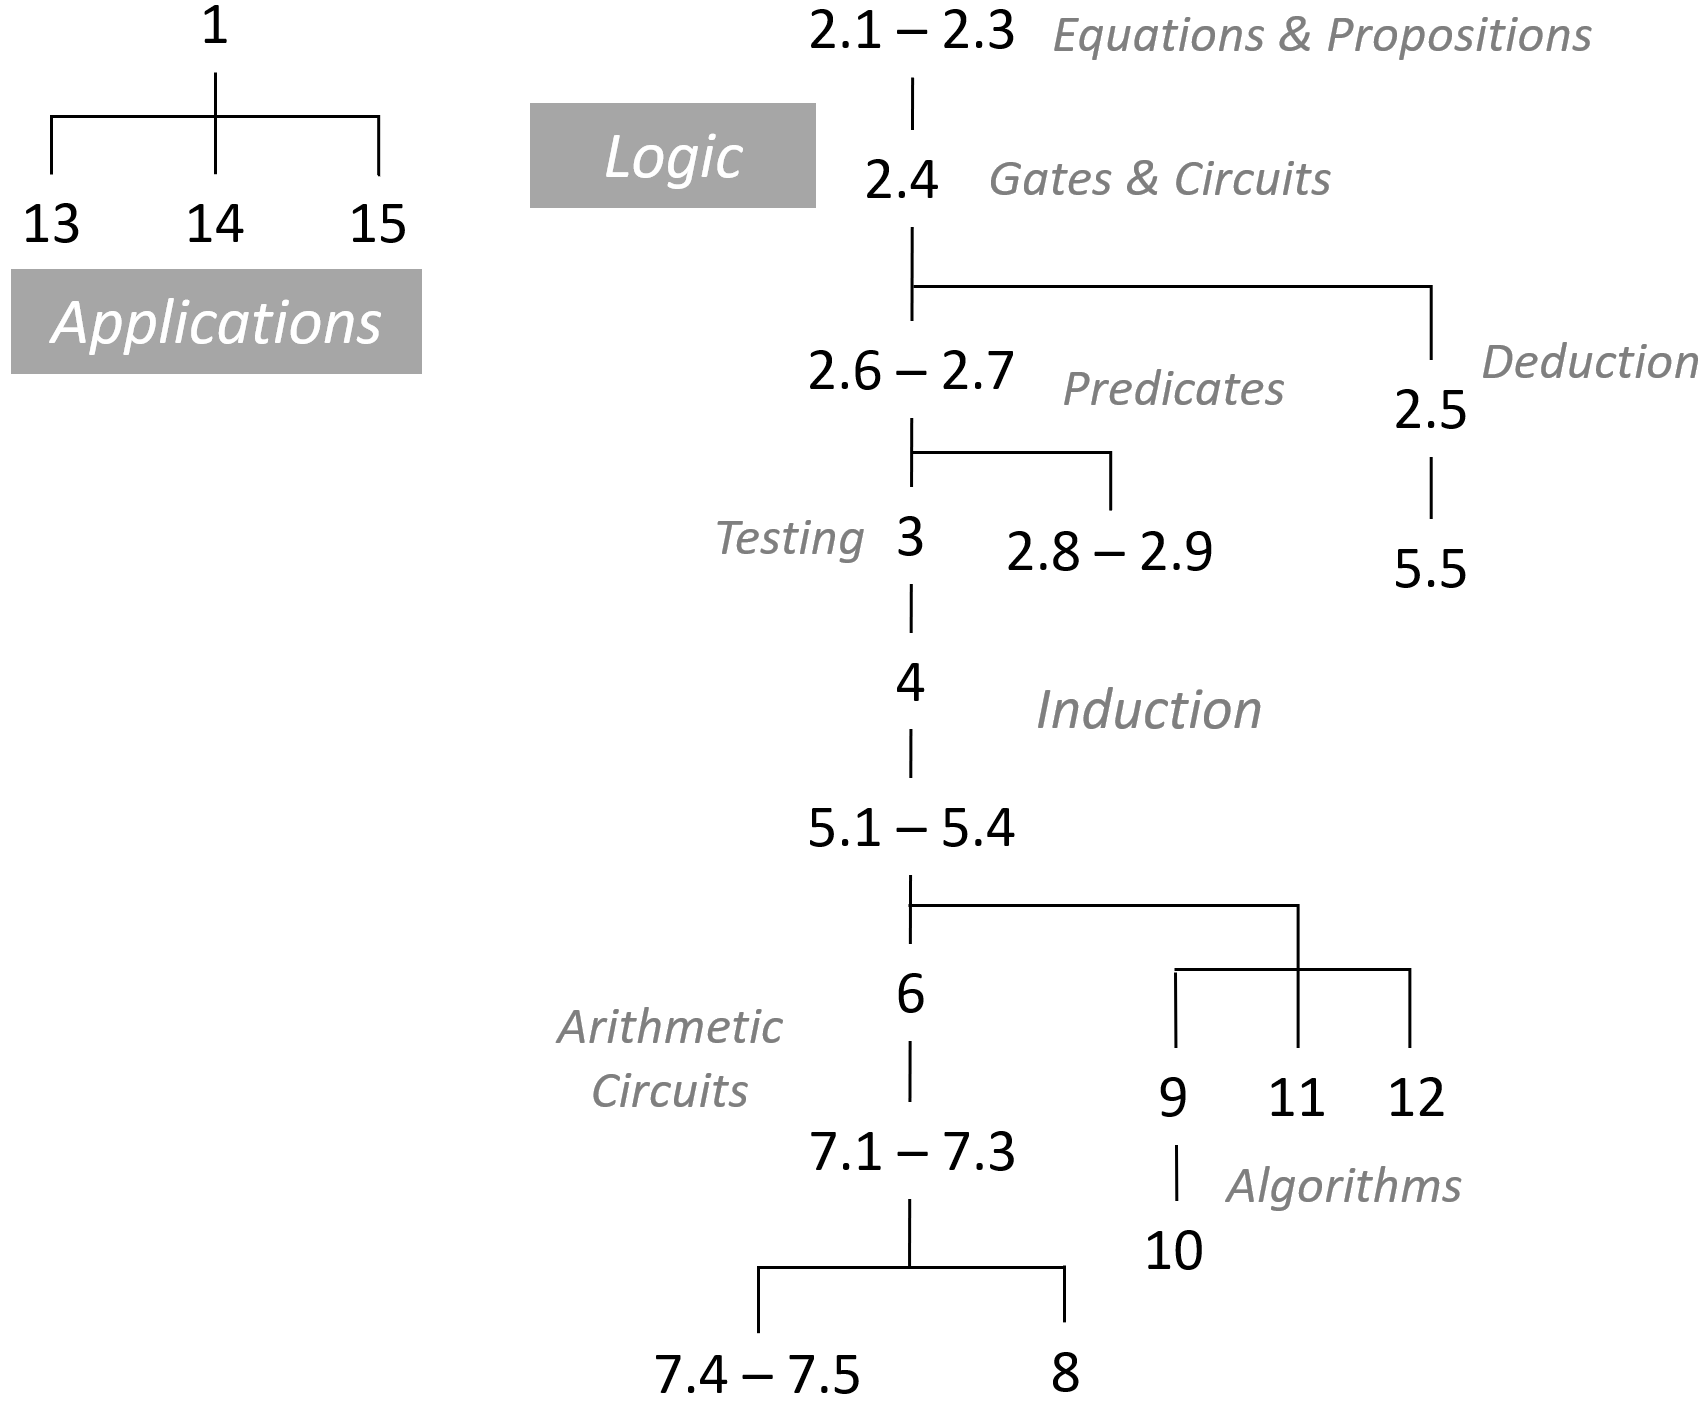
\includegraphics[scale=0.25]{images/roadmap.png}
\end{center}


%%% Local Variables:
%%% mode: latex
%%% TeX-master: "book"
%%% End:
